\documentclass[12pt]{article}

% Solutions toggle
\newif\ifsolutions
\solutionsfalse
%% \solutionstrue

% ASSIGNMENT NUMBER
\newcommand{\hwnumber}{6}
\newcommand{\booksection}{}
\newcommand{\duedate}{}
% -------------

%%% Packages
\usepackage[margin=1in, footskip=24pt, headheight=24pt]{geometry}
\usepackage{amsmath, amssymb, amsthm, graphicx}
\usepackage{mathtools}
\DeclarePairedDelimiter\ceil{\lceil}{\rceil}
\DeclarePairedDelimiter\floor{\lfloor}{\rfloor}
\usepackage[colorlinks, urlcolor=blue]{hyperref}
\usepackage{color}
\usepackage{comment}
\usepackage{enumerate}
\usepackage{lastpage}
\usepackage{multirow, multicol}
\usepackage{tikz}
\usetikzlibrary{matrix,decorations.text,decorations.pathmorphing,decorations.markings,arrows,calc,shapes.geometric,patterns,shadows,intersections,decorations.markings,decorations.pathreplacing,decorations.pathreplacing,backgrounds,angles,quotes}
\usepackage{pgfplots}
\pgfplotsset{compat=1.16}

\usepackage{fancyhdr}

\pagestyle{fancy}
%% \renewcommand{\familydefault}{\sfdefault}

\newcommand{\R}{\mathbb{R}}
\newcommand{\ddx}{\frac{d}{dx}}

\global\long\def\V#1{\boldsymbol{#1}} %vector
\global\long\def\M#1{\boldsymbol{#1}} %matrix

\global\long\def\D#1{\Delta#1} %\D{t} for time step size
\global\long\def\d#1{\delta#1} %\d{t} for small increment

\global\long\def\norm#1{\left\Vert #1\right\Vert }
\global\long\def\abs#1{\left|#1\right|}

\global\long\def\grad{\M{\nabla}}
\global\long\def\av#1{\left\langle #1\right\rangle }

% HEADER MACROS
\newcommand{\term}{Spring 2022 \& 2023}
\newcommand{\coursename}{Intro Math Modeling}
\newcommand{\coursenumber}{MATH-UA 251}
\newcommand{\course}{\coursename \ (\coursenumber)}

\fancyhead[RO]{\term}
\fancyhead[LO]{\course}
% -------------

%%% Theorem Styles
\theoremstyle{definition}
\newtheorem{ex}{Exercise}

%%%%%%%%%%%%%%%%%%%%%%%% Solutions %%%%%%%%%%%%%%%%%%%%%%%%%%%%%
% \begin{solution} and \begin{answerspace} must be at the beginning of the line.
% Doesn't work inside the \myversions command. Use if statements instead.
% No underscores in comment names

\ifsolutions
\newenvironment{solution}{\color{blue}}{} \excludecomment{answerspace} \newenvironment{notes}{\color{red} \noindent Grading Notes:}{}
\else
\excludecomment{notes} \excludecomment{solution} \includecomment{answerspace} 
\fi
%%%%%%%%%%%%%%%%%%%% End Solutions %%%%%%%%%%%%%%%%%%%%%%%e}


\begin{document}
% HEADER
\begin{center}
%% \ifsolutions
%%   \textbf{\Large Homework \hwnumber\ - \booksection\ (Solutions)}\\
%% \else
%%   \textbf{\Large Homework \hwnumber\ - \booksection}\\
%% \fi
\ifsolutions
  \textbf{\Large Homework \hwnumber\ (Solutions)}\\
\else
  \textbf{\Large Homework \hwnumber}\\
\fi
\vspace{12pt}
Due date: someday, sometime! \duedate

Submit on NYU Brightspace.
\end{center}

%% \noindent Please give complete, well-written solutions to the following exercise. Provide sufficient justification and explanation for a classmate who has not worked on the exercise to understand your solution.


\begin{ex}
  
  [100 pts] For each of the following affairs, find the eigenvalues and eigenvectors, and sketch (by hand), qualitatively, all possible phase portraits (if applicable, depending on the signs and relative sizes of $a$ and $b$). Do \textbf{NOT} use computer to make the plots. Specify the stability of the origin $[R,J]=[0,0]$ (stable node, saddle point, center (for closed orbits), or stable/unstable spirals). Your sketches should show the important qualitative features of each case. Interpret the phase portraits.
  \begin{enumerate}[(i)]\setlength{\itemsep}{0pt}
  \item (35 pts) $\dot{R}=J,\;\dot{J}=-R+J$
  \item (35 pts) $\dot{R}=aJ,\;\dot{J}=bR,\;(a,b\neq 0)$
  \item (30 pts) $\dot{R}=aR+bJ,\;\dot{J}=bR+aJ,\;(a<0,\;b>0,\;a^2=b^2)$
  \end{enumerate}

\noindent\textbf{\textcolor{red}{notes:} }Solutions without details of the work and interpretation of the results will not receive full credits. 

\begin{solution}
  \begin{enumerate}[(i)]\setlength{\itemsep}{0pt}
  \item $\dot{R}=J,\;\dot{J}=-R+J$

  \begin{equation*}
    A=
    \begin{bmatrix}
      0 & 1\\
      -1 & 1
    \end{bmatrix}
    \Rightarrow \det\left(
    \begin{bmatrix}
      -\lambda & 1\\
      -1 & 1-\lambda
    \end{bmatrix}
    \right)=0\Rightarrow \lambda^2-\lambda+1=0\Rightarrow \lambda=\frac{1}{2}\pm i\frac{\sqrt{3}}{2}.
  \end{equation*}

  The corresponding eigenvectors are
  \begin{align*}
    &\begin{bmatrix}
      -\lambda & 1\\
      -1 & 1-\lambda
    \end{bmatrix}
    \begin{bmatrix}
      \alpha\\
      \beta
    \end{bmatrix}
    =0\Rightarrow V=
    \begin{bmatrix}
      1\\
      \lambda
    \end{bmatrix},\\
    &\lambda_1=\frac{1}{2}+i\frac{\sqrt{3}}{2}\Rightarrow V_1=\begin{bmatrix}1\\\frac{1}{2}+i\frac{\sqrt{3}}{2}\end{bmatrix},\\
    &\lambda_2=\frac{1}{2}-i\frac{\sqrt{3}}{2}\Rightarrow V_2=\begin{bmatrix}1\\\frac{1}{2}-i\frac{\sqrt{3}}{2}\end{bmatrix}.
  \end{align*}
    
  The origin is an unstable spiral since the real part of the eigenvalues is positive (see \autoref{Figure_i}). To find out if the flow is clockwise or counter-clockwise, we test a point like $(R,J)=(1,0)$ (on the $R$ axis in the 2D plot of $J$ versus $R$) which yields $(\dot{R},\dot{J})=(J,-R+J)=(0,-1)$. Therefore, the velocity vector is pointing downward, and hence, the flow pattern is clockwise. We see that regardless of the starting point, there is an everlasting cycle of love and hate for Romeo and Juliet. As time goes on, the magnitude of the love and hate they experience intensifies! This is not recommended!
    
  \begin{figure}[h]
    \centering
    \resizebox{0.4\textwidth}{!}{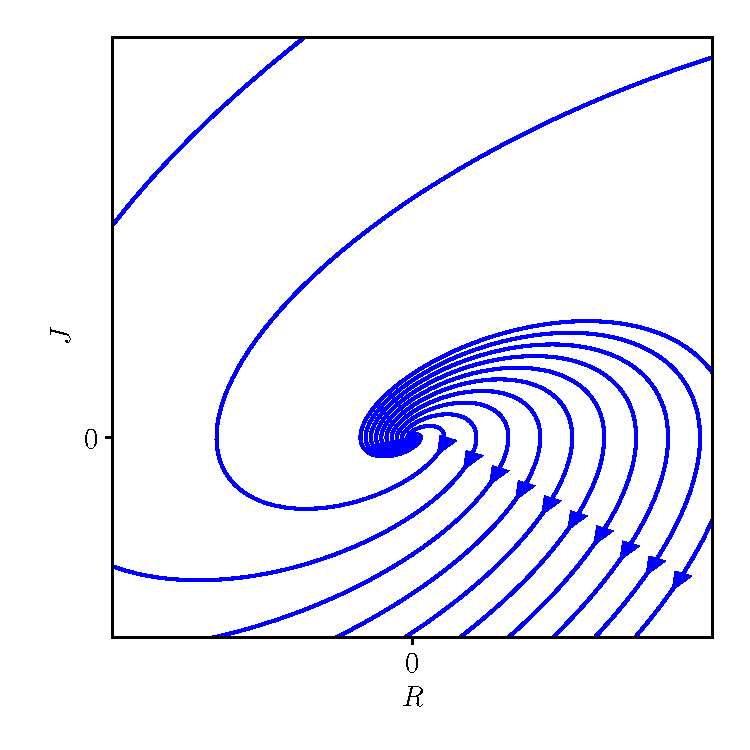
\includegraphics{HW6_i_plot.pdf}}
    \caption{(i) origin is an unstable spiral.}
    \label{Figure_i}
  \end{figure}

  \item $\dot{R}=aJ,\;\dot{J}=bR,\;(a,b\neq 0)$

  \begin{equation*}
    A=
    \begin{bmatrix}
      0 & a\\
      b & 0
    \end{bmatrix}
    \Rightarrow \det\left(
    \begin{bmatrix}
      -\lambda & a\\
      b & -\lambda
    \end{bmatrix}
    \right)=0\Rightarrow \lambda^2-ab=0\Rightarrow \lambda=\pm\sqrt{ab}=
    \begin{cases}
      \pm\sqrt{ab} & ab>0,\\
      \pm i\sqrt{\lvert ab\rvert} & ab<0,
    \end{cases}
  \end{equation*}
  with the following eigenvectors:
  \begin{equation*}
    \begin{bmatrix}
      -\lambda & a\\
      b & -\lambda
    \end{bmatrix}
    \begin{bmatrix}
      \alpha\\
      \beta
    \end{bmatrix}
    =0\Rightarrow V=
    \begin{bmatrix}
      1\\
      \lambda/a
    \end{bmatrix}.
  \end{equation*}

  When $ab>0$, the corresponding eigenvectors are
  \begin{align*}
    &\lambda_1=+\sqrt{ab}\Rightarrow V_1=
    \begin{cases}
      \left[1,+\sqrt{b/a}\right]^T & a,b>0\\
      \left[1,-\sqrt{b/a}\right]^T & a,b<0
    \end{cases}\\
    &\lambda_2=-\sqrt{ab}\Rightarrow V_2=
    \begin{cases}
      \left[1,-\sqrt{b/a}\right]^T & a,b>0\\
      \left[1,+\sqrt{b/a}\right]^T & a,b<0\\
    \end{cases}
  \end{align*}
  Note that here we used the fact that if $x<0$, then $x=-|x|$, e.g., when $a<0$, $\sqrt{ab}/a=-\sqrt{ab}/|a|=-\sqrt{b/a}$. The origin will be a saddle point regardless: both eigenvalues are real and $\lambda_1>0,\lambda_2<0$. But the direction of trajectories is determined by the sign and $a$ (or equivalently $b$). \autoref{Figure_ii_saddle} shows the case when $a$ and $b$ are both positive. The phase portrait remains qualitatively the same when $a$ and $b$ are both negative, but all of the directions will be reversed. This has an important consequence on the outcome of the relationship though! When $a,b>0$ we have either $R\to+\infty,J\to+\infty$ (love fest) or $R\to-\infty,J\to-\infty$ (war!). When $a,b<0$, however, the outcome is either $R\to+\infty,J\to-\infty$ or $R\to-\infty,J\to+\infty$, both of which are identically disastrous!

  When $ab<0$, the eigenvectors become
  \begin{align*}
    &\lambda_1=+i\sqrt{\lvert ab\rvert}\Rightarrow V_1=
    \begin{cases}
      \left[1,+i\sqrt{\lvert b/a\rvert}\right]^T & a>0\\
      \left[1,-i\sqrt{\vert b/a\rvert}\right]^T & a<0
    \end{cases}\\
    &\lambda_2=-i\sqrt{\lvert ab\rvert}\Rightarrow V_2=
    \begin{cases}
      \left[1,-i\sqrt{\lvert b/a\rvert}\right]^T & a>0\\
      \left[1,+i\sqrt{\lvert b/a\rvert}\right]^T & a<0\\
    \end{cases}
  \end{align*}
  The origin will be a center: both eigenvalues are complex with no real part (see \autoref{Figure_ii_center}). To find out if the flow is clockwise or counter-clockwise, we test a point like $(R,J)=(1,0)$ which yields $(\dot{R},\dot{J})=(aJ,bR)=(0,b)$. Therefore, the velocity vector is pointing downward (clockwise flow) and upward (counter-clockwise flow) for $b<0$ ($a>0$) and $b>0$ ($a<0$), respectively. Figure below shows an example for which $a=1,b=-1$. Regardless, the phase portrait shows closed orbits which indicates endless cycles of love and hate. They at least love each other one quarter of the time.

  \begin{figure}[h]
  \centering
  \begin{minipage}[t]{0.45\textwidth}
    \centering
    \resizebox{1\textwidth}{!}{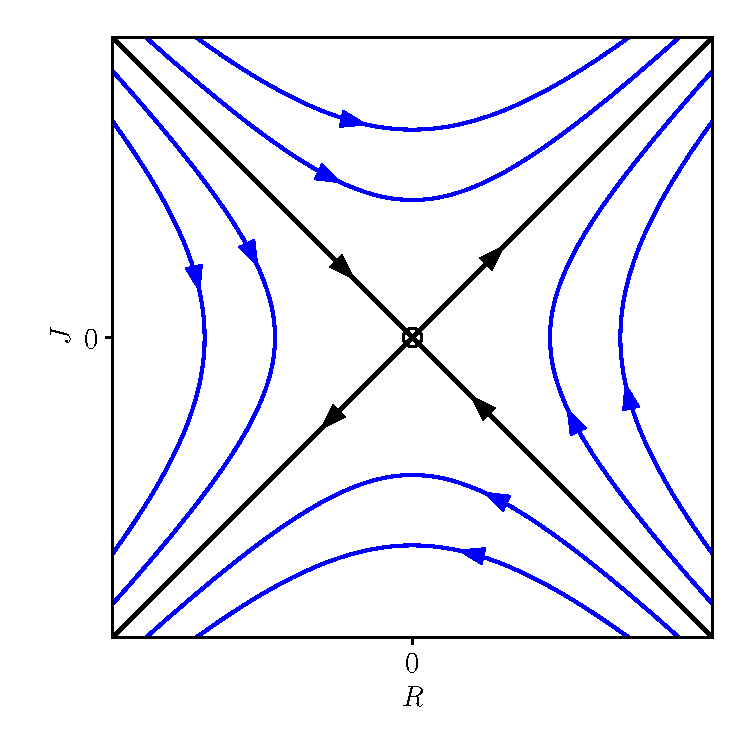
\includegraphics{HW6_ii_plot_saddle.pdf}}
    \caption{(ii) $a>0,b>0$ ($a=1,\;b=1$): origin is a saddle point. All directions will be reversed for $a<0,b<0$.}
    \label{Figure_ii_saddle}
  \end{minipage}\hfill
  \begin{minipage}[t]{0.45\textwidth}
    \centering
    \resizebox{1\textwidth}{!}{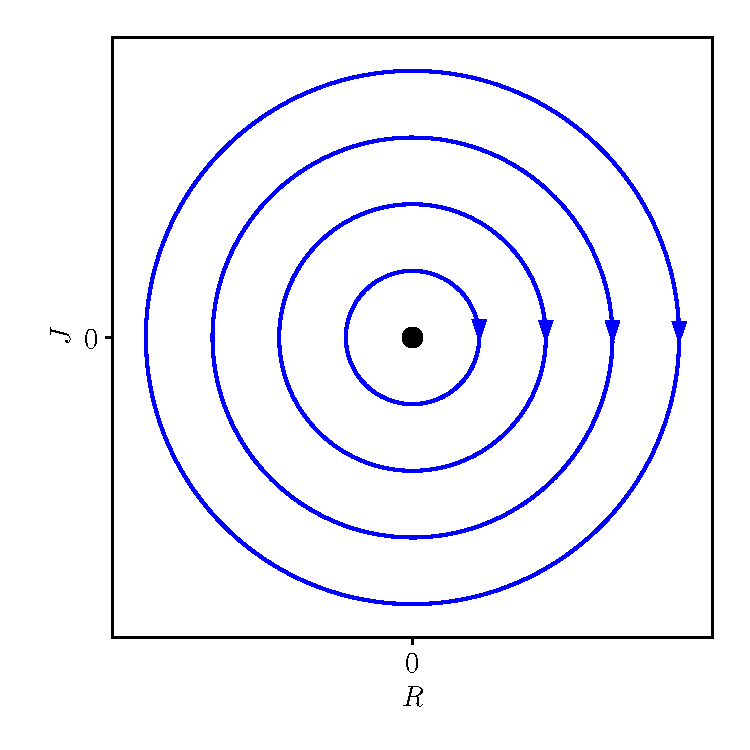
\includegraphics{HW6_ii_plot_center.pdf}}
    \caption{(ii) $ab<0$ ($a=1,\;b=-1$): origin is a center. The direction of rotation will be reversed for $a<0,b>0$.}
    \label{Figure_ii_center}
  \end{minipage}
  \end{figure}

  \item $\dot{R}=aR+bJ,\;\dot{J}=bR+aJ,\;(a<0,\;b>0,\;a^2=b^2)$

  \begin{equation*}
    A=
    \begin{bmatrix}
      a & b\\
      b & a
    \end{bmatrix}
    \Rightarrow \det\left(
    \begin{bmatrix}
      a-\lambda & b\\
      b & a-\lambda
    \end{bmatrix}
    \right)=0\Rightarrow (a-\lambda)^2-b^2=0\Rightarrow \lambda=a\pm b.
  \end{equation*}

  The corresponding eigenvectors are
  \begin{align*}
    &\begin{bmatrix}
      a-\lambda & b\\
      b & a-\lambda
    \end{bmatrix}
    \begin{bmatrix}
      \alpha\\
      \beta
    \end{bmatrix}
    =0\Rightarrow V=
    \begin{bmatrix}
      1\\
      (\lambda-a)/b
    \end{bmatrix},\\
    &\lambda_1=a+b\Rightarrow V_1=\begin{bmatrix}1\\1\end{bmatrix},\\
    &\lambda_2=a-b\Rightarrow V_2=\begin{bmatrix}1\\-1\end{bmatrix}.
  \end{align*}
    
  If $a^2=b^2$, then $\lambda_1=0$ and $\lambda_2<0$. This implies that the system does not change in the eigendirection corresponding to $V_1$. We end up with a line of fixed points on the eigendirection. (see \autoref{Figure_iii}). An interpretation is that regardless of the initial conditions, the outcome of the love affair lies on the $J=R$ line: they will equally love or hate each other.
  
  \begin{figure}[h]
    \centering
    \resizebox{0.4\textwidth}{!}{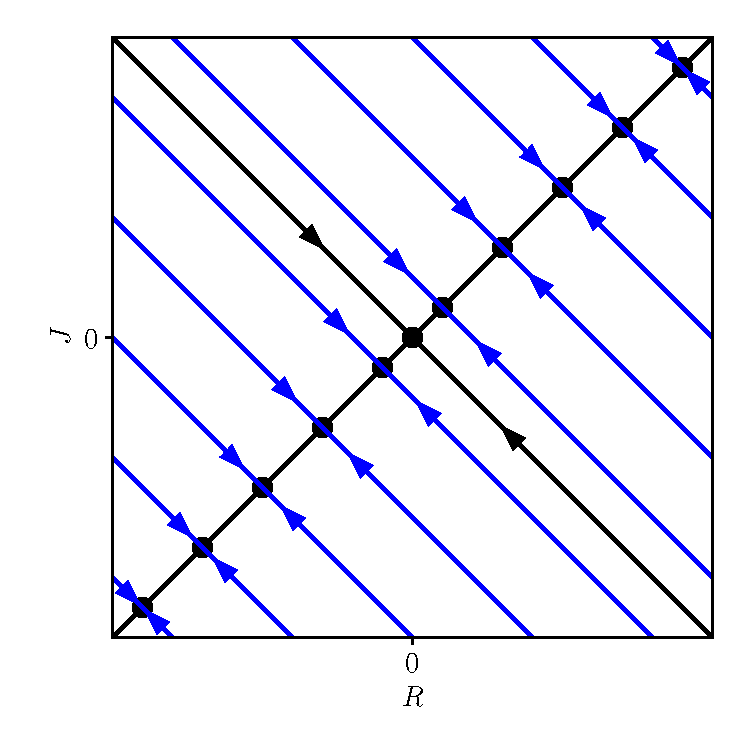
\includegraphics{HW6_iii_plot.pdf}}
    \caption{(iii) there is a line of fixed points along the eigendirection of $\lambda_1=0,V_1=[1,1]^T$.}
    \label{Figure_iii}
  \end{figure}

  
  \end{enumerate}
  
\end{solution}
\end{ex}


\end{document}
